\documentclass[12pt,3p]{article}
\usepackage[T1]{fontenc}
\usepackage[utf8]{inputenc}
\usepackage[english]{babel}
\usepackage[margin=0.75in]{geometry}
\usepackage{amsmath}
\usepackage{mathtools}
\usepackage{enumitem}
\usepackage{physics}
\usepackage{bm}
\usepackage[font=small]{caption}

\usepackage[round,numbers]{natbib}
\usepackage[colorlinks = false]{hyperref}

\begin{document}

\title{\Large{FEniCS: Three FEniCS Demonstrations related to Poisson's Equations} \vspace{-5ex}}
\author{Ida Ang, Edited \today}
\date{\vspace{-5ex}}
\maketitle

\tableofcontents
\newpage
%=====================================================================
%=====================================================================
%=====================================================================
\section{Problem Definition}
\vspace{-2ex}
This document demonstrates three implementations for Poisson's equations that exists in the \href{https://fenicsproject.org/olddocs/dolfin/1.4.0/python/demo/index.html}{Programmer's reference for Dolfin (Python)}. The first and simplest demonstration of the Poisson Equation is given in the programmer's reference demonstration number 16, \href{https://fenicsproject.org/olddocs/dolfin/1.3.0/python/demo/documented/poisson/python/documentation.html}{Poisson Equation Demonstration}. The second demonstration is the \href{https://fenicsproject.org/olddocs/dolfin/1.4.0/python/demo/documented/periodic/python/documentation.html}{Poisson's Equation with periodic boundary condition}.The third demonstration demonstrates how to solve for the \href{https://fenicsproject.org/olddocs/dolfin/1.4.0/python/demo/documented/mixed-poisson/python/documentation.html}{mixed formulation for Poisson's equation}. 

There are two keys goals to this document: 1) Fix any errors from documents that have not been updated to the last FEniCS stable version, and 2) provide more details of the theory and conversion from the strong form, or partial differential equations, to the weak form, or integral equation. This document provides the detailed steps for beginners who might have just been exposed to indicial notation. In direct notation, bolded uncapitalized notation refers to vectors, unbolded notation refers to scalar variables.
 
%=====================================================================
%=====================================================================
%=====================================================================
\section{Formulations}
\vspace{-2ex}
The simplest formulation for Poisson's problem involves solving for one variable, $u$, which is known as a scalar field of scalar potential. The Poisson's equation shows up in many contexts, and the variable $u$ could be the concentration of some chemical solute, as a function of position x, or the temperature $T$ in some heat conducting medium. Classically, the equation can be referred to as the divergence of the gradient of some scalar field which then returns a scalar, some source term $f$.
\begin{subequations}\label{EqPoisson}
\begin{align}
\nabla \cdot \nabla u = \nabla^2 u = \Delta u = f \quad \text{in } \Omega 
\end{align}
\end{subequations}
It can also be referred to as the Laplacian of the variable field, where several notations are listed in Eq. \ref{EqPoisson}.


%=====================================================================
%=====================================================================
\subsection{Poisson's Equation}
\vspace{-1ex}
The first setup involves Poisson's equation solved within a two dimensional square domain $\Omega$ . The boundary consists of the Dirichlet (D) and Neumann (N) boundaries combined together: $\partial \Omega = \Gamma_D \cup \Gamma_N$. 
\begin{subequations}\label{EqProbDef1}
\begin{align}
- \nabla^2 u &= f(x,y) \quad \text{in } \Omega \\
		u &= 0 \quad \quad \quad \text{on } \Gamma_D \\
\nabla u \cdot \mathbf{n} = \pdv{u}{\mathbf{n}} &= g \quad \quad \quad \text{on } \Gamma_N
\end{align}
\end{subequations}
The Dirichlet boundary condition (BC) is the essential boundary condition applied within the function space, while the Neumann boundary condition is the natural boundary condition which is subsumed into the variational weak form. The gradient of scalar field gives a vector, which can be dotted with the normal vector to the boundary $\Gamma_N$, which is equivalent to some boundary term $g$. The source term $f$ and boundary term $g$ can be defined as follows:
\begin{subequations}\label{EqSourceBoundTerm}
\begin{align}
f(x,y) &= 10 e^{-\frac{x^2 + y^2}{0.02}} \\
g(x) &= \sin(5x)
\end{align}
\end{subequations} 
To see the relationship in Eq. \ref{EqProbDef1}c, we can rewrite the Neumann boundary condition in indicial or Einstein notation, where $\nabla u = \pdv{u}{x_i} \mathbf{e_i} $
\begin{align*}
\nabla u \cdot \mathbf{n} 
	&= \pdv{u}{x_i} \mathbf{e_i} \cdot n_k \mathbf{e_k} \\
	&= \pdv{u}{x_i} n_k (\mathbf{e_i} \cdot \mathbf{e_k}) \\
	&= \pdv{u_j}{x_i} n_k \delta_{ik} \\
\nabla u \cdot \mathbf{n} &= \pdv{u}{x_i} n_i = g
\end{align*}
Therefore the Neumann boundary condition can be written as,
\begin{equation}\label{EqNBoundInd}
\pdv{u}{x_i} n_i  = g
\end{equation}
where Eq. \ref{EqProbDef1}c is the same as Eq. \ref{EqNBoundInd}.
%---------------------------------------------------------------------------------------------------------------------------------------------------
The next section goes through the conversion of the partial differential equation to the integral or weak form. First, write the laplacian in indicial notation: 
\begin{align*}
\nabla u 
	&= \pdv{u}{x_i} \mathbf{e_i} \\
\nabla \cdot \nabla u 
	&= \pdv{}{x_j} \mathbf{e_j} \cdot \pdv{u}{x_i} \mathbf{e_i} \\
	&= \pdv{u}{x_j}{x_i} \big( \mathbf{e_j} \cdot \mathbf{e_i} \big) \\
\nabla \cdot \nabla u 
	&= \pdv[2]{u}{x_i} 
\end{align*}
Therefore, we can write Eq. \ref{EqProbDef1}
\begin{equation}\label{EqProbDef1Ind}
- \pdv[2]{u}{x}  = f
\end{equation}
Multiply Eq. \ref{EqProbDef1Ind} by scalar test function, $v$: 
\begin{align}\label{EqBefIntParts}
\begin{split}
- \pdv[2]{u}{x} v 
	&= f v \quad \text{Integrate over domain } \Omega\\
- \int_{\Omega} \pdv[2]{u}{x} v \,d {x} 
	&= \int_{\Omega} f v \, d {x} 
\end{split}
\end{align}
Use integration by parts,
\begin{equation}\label{EqIntParts1}
(fg)' = f'g + fg' \rightarrow f'g = (fg)' - fg' \rightarrow f''g = (f'g)' - f'g'
\end{equation}
Where we can substitute $f'' = \pdv[2]{u}{x_i} $ and $g = v$ into Eq. \ref{EqIntParts1}
\begin{equation*}
\pdv[2]{u}{x_i} v = \nabla \cdot \bigg( \pdv{u}{x_i} v \bigg) - \pdv{u}{x} \pdv{v}{x}
\end{equation*}
Change signs and substitute into Eq. \ref{EqBefIntParts}
\begin{align*}
- \int_{\Omega} \nabla \cdot \bigg( \pdv{u}{x} v \bigg) \, d{x} 
+ \int_{\Omega} \pdv{u}{x} \pdv{v}{x} \, d {x} 
	&= \int_{\Omega} f v  \, d{x} \quad \text{Use divergence theorem on first term}\\
- \int_{\partial \Omega}  \bigg( \pdv{u}{x} \mathbf{n} \bigg)  \, v  \, d{s} 
+ \int_{\Omega} \pdv{u}{x} \pdv{v}{x} \, d {x} 
	&= \int_{\Omega} f v \, d{x} \quad \text{Recognize Neumann BC Eq. \ref{EqNBoundInd} on first term} \\
- \int_{\Gamma_N}  g v \, d{s}  
+ \int_{\Omega} \pdv{u}{x} \pdv{v}{x} \, d{x}  
	&= \int_{\Omega} f v \, d{x}  \quad \text{$u = 0$ on Dirichlet boundary} 
\end{align*}
Therefore, the weak form in indicial and direct notation
\begin{subequations}\label{EqWeakForm}
\begin{align}
\int_{\Omega} \pdv{u}{x} \pdv{v}{x} \, d{x}  
	&= \int_{\Omega} f v \, d{x}  + \int_{\Gamma_N}  g v \, d {s} \\
\int_{\Omega} \nabla u \cdot \nabla v \, d{x} 
	&= \int_{\Omega} f \cdot v \, d{x} + \int_{\Gamma_N} g \cdot v \, d{x} 
\end{align}
\end{subequations}

\subsection{Poisson's Equation with Periodic Boundary Condition}
This formulation follows as in the section above, except no Neumann Boundary condition is applied. The same square domain, $\Omega$ is specified where the boundary, $\partial \Omega=\Gamma_D \cup \Gamma_P$, consists of the Dirichlet and periodic boundary conditions. 
\begin{subequations}\label{EqStrongFormPBC}
\begin{align}
-\nabla \cdot(\nabla u) & =f \quad \text { in } \Omega, \\
u & =0 \quad \text { on } \Gamma_D, \\
u(0, y) & =u(1, y) \quad \text { on } \Gamma_P .
\end{align}
\end{subequations}
A Dirichlet BC is applied on the top and bottom surface of the square. A periodic boundary condition means that there is some periodicity to the solutions at the boundary. In this demonstration, the solution for the potential field, $u$, on the right boundary is mapped to the left boundary. The implemented weak form looks as follows:
\begin{equation}\label{EqWeakFormWoNeumann}
\int_{\Omega} \nabla u \cdot \nabla v \, d{x} = \int_{\Omega} f \cdot v \, d{x} 
\end{equation}
Note, that the source term in this case is changed (see implementation section). 


%=====================================================================
%=====================================================================
\subsection{Mixed formulation for Poisson Equation}
\vspace{-1ex}
An alternate formulation for the Poisson's equation involves introduction of a vector field, $\mathbf{q}$, the heat flux, through Fourier's Law. Fourier's law assumes that the heat flux is proportional to the gradient of the negative temperature
\begin{align}\label{EqFourierLaw}
\begin{split}
\bm{q} &= - \kappa \nabla u \quad \kappa = -1 \\
\bm{q} &= \nabla u 
\end{split}
\end{align}
In this particular problem, the heat conductivity, $\kappa= -1$,  and $u$ is the temperature field. 

Consider a model for the temperature $u$, in a body occupying a domain $\Omega$ subject to a heat source, f. It follows by conservation of energy that the outflow of energy over the boundary $\partial \Omega$ must be balanced by the energy emitted by the heat source $f$: 
\begin{align}\label{EqProbDef2}
\begin{split}
\int_{\partial \Omega} \bm{q} \cdot \mathbf{n} \, d {s} &= - \int_{\Omega} f d {x} \quad \text{Use the Gaussian theorem} \\
\int_{\Omega} \nabla \cdot \bm{q} \, d\mathbf{x} &= - \int_{\Omega} f \, d \mathbf{x} \\
\nabla \cdot \bm{q} &= - f \quad \text{in } \Omega
\end{split}
\end{align}
Note, the divergence of a vector field gives a scalar. We can thus substitute this into Poisson's equation Eq. \ref{EqPoisson}. 
\begin{align*}
- \nabla \cdot (\nabla u) &= f \quad \text{Substitute Eq. \ref{EqFourierLaw}} \\
- \nabla \cdot \mathbf{q}  &= f
\end{align*}

The strong form can thus be stated alongside the Neumann (Natural) and Dirichlet (Essential) boundary condition enforced on $\Gamma_N$ and $\Gamma_D$ respectively, 
\begin{subequations}\label{EqStrongForm2}
\begin{align}
- \nabla \cdot \bm{q} &= f \quad \text{in } \Omega \\
\bm{q} - \nabla u &= 0 \indent \text{in } \Omega \\
u &= u_o \indent \text{on } \Gamma_D \\
\bm{q} \cdot \bm{n} &= g \indent \text{on } \Gamma_N
\end{align}
\end{subequations}
where we are solving for the scalar temperature field $u$ and the vector field of heat flux $\mathbf{q}$ in their respective function spaces. In this case, what used to be the Neumann boundary condition, the flux condition in Eq. \ref{EqStrongForm2}d, becomes a Dirichlet or Essential boundary condition, because it must be now enforced in the function space. Meanwhile what used to be the Dirichlet boundary condition becomes the Neumann boundary condition, which must be applied in the weak form. 

See the derivation for the next section. We have two partial differential equations in Eq. \ref{EqStrongForm2}, leading to the introduction of two different test functions, $\bm{\tau}$ and $v$. 

%=====================================================================
\subsubsection{Fourier's Law to Weak Form}
Write Eq. \ref{EqFourierLaw} in indicial 
\begin{align*}
-\pdv{}{x_j} \mathbf{e_j} \cdot q_i e_i &= f \\
-\pdv{q_i}{x_j} \delta_{ji} &= f \\
-\pdv{q_i}{x_i}  &= f
\end{align*}
Next, multiply this with a scalar test function 
\begin{align*}
-\pdv{q_i}{x_i} v &= f v  \quad \text{Integrate over domain}\\
- \int_{\Omega} \pdv{q_i}{x_i} v \, d x &= \int_{\Omega} f v \, dx 
\end{align*}
Change to direct notation, leaving the following variational (weak) equation. 
\begin{subequations}\label{EqWeakForm2}
\begin{align}
- \int_{\Omega} \pdv{q_i}{x_i} v \, d x &= \int_{\Omega} f v \, dx \\
- \int_{\Omega} (\nabla \cdot \bm{q}) v \, dx &=  \int_{\Omega} f v \, dx
\end{align}
\end{subequations}

%=====================================================================
\subsubsection{Weak Form 2}
Convert Eq. \ref{EqProbDef2} to indicial notation: 
\begin{align}\label{EqParts}
\begin{split}
\mathbf{q} = \nabla u \rightarrow q_{i} \mathbf{e_i} &= \pdv{u}{x_i} \mathbf{e_i} \quad \text{Multiply with test function } \bm{\tau} \\
q_{i} \mathbf{e_i} \cdot \tau_k \mathbf{e_k} &= \pdv{u}{x_i} \mathbf{e_i} \cdot \tau_k \mathbf{e_k} \\
q_{i} \tau_k \delta_{ik} &= \pdv{u}{x_i} \tau_k \delta_{ik} \\
q_{i} \tau_i &= \pdv{u}{x_i} \tau_9 \quad \text{Integrate over domain} \\
\int_{\Omega} q_{i} \tau_i  \, dx &= \int_{\Omega} \pdv{u}{x_i} \tau_i \, dx
\end{split}
\end{align}
Use integration by parts on the right hand side 
\begin{equation}\label{EqIntParts2}
(fg)' = f'g + fg' \rightarrow f'g = (fg)' - fg'
\end{equation}
Where we can substitute $f' = \pdv{u}{x_i} $ and $g = \tau_i$ into Eq. \ref{EqIntParts2}
\begin{equation*}
\pdv{u}{x_i} \tau_i = (u \tau_i)_{,i} - u \pdv{\tau_i}{x_i}
\end{equation*}
Substitute into right hand side of Eq. \ref{EqIntParts2}
\begin{align*}
\int_{\Omega} q_{i} \tau_i  \, dx 
	&= \int_{\Omega} \pdv{u}{x_i} \tau_i \, dx \\
	&=  \int_{\Omega} (u  \tau_i)_{,i} \, dx 
	- \int_{\Omega} u \pdv{\tau_i}{x_j} \, dx \quad \text{Use divergence theorem} \\
\int_{\Omega} q_{i} \tau_i  \, dx 
	&= \int_{\partial \Omega} u \, \tau_j n_i \, dx - \int_{\Omega} u \pdv{\tau_i}{x_i} \, dx
\end{align*}
Therefore, we have the second weak forms in both indicial and direct notation below.
\begin{subequations}\label{EqWeakForm3}
\begin{align}
\int_{\Omega} q_{i} \tau_i  \, dx + \int_{\Omega} u \pdv{\tau_i}{x_i} \, dx 
	&= \int_{\partial \Omega} u \, \tau_j n_i \, dx \\
\int_{\Omega} \bm{q} \cdot \bm{\tau} \, dx + \int_{\Omega} u \, (\nabla \cdot \bm{\tau}) \, dx &= \int_{\Gamma} u \,(\bm{\tau} \cdot \bm{n})  \, ds 
\end{align}
\end{subequations}
Therefore, combining Equations \ref{EqWeakForm2} and \ref{EqWeakForm3}, the weak form can be phrased as such: Find $(\bm{\tau}, \, u) \in (\Sigma_g \times V)$
\begin{subequations}\label{EqWeakFormTotal}
\begin{align}
\int_{\Omega} \bm{q} \cdot \bm{\tau} \, dx + \int_{\Omega} (\nabla \cdot \bm{\tau}) \bm{u} \, dx &= \int_{\Gamma} (\bm{\tau} \cdot \bm{n}) \bm{u} \, ds \indent \forall \bm{q} \in \Sigma \\
\int_{\Omega} (\nabla \cdot \bm{q}) v \, dx &= - \int_{\Omega} fv \, d x \indent \forall v \in V
\end{align}
\end{subequations}


%=====================================================================
%=====================================================================
%=====================================================================
\section{FEniCS Implementation}
\vspace{-2ex}

%=====================================================================
%=====================================================================
\subsection{Poisson's Equation}
\vspace{-1ex}
One key change from the original is the change in the mesh. Instead of using \\
{\fontfamily{qcr}\selectfont
mesh = UnitSquareMesh(32, 32) \\ \\
} 
The mesh is set with \\ 
{\fontfamily{qcr}\selectfont
mesh = RectangleMesh(Point(-0.5, -0.5), Point(0.5, 0.5), int(N), int(N)) \\
} 
which simply changes the origin to the center of the square. The boundaries are also specified with the following class, \\
{\fontfamily{qcr}\selectfont
class boundary(SubDomain): \\
\indent def inside(self, x, on\_boundary): \\
\indent \indent return x[0] < -0.5 + DOLFIN\_EPS or x[0] > 0.5 - DOLFIN\_EPS \\ 
}
which specifies the left hand side and the right hand side of the square for the Dirichlet boundary conditions. {\fontfamily{qcr}\selectfont DOLFIN\_EPS } is simply a machine precision-like number. The boundary can be saved to a file to determine whether the boundaries are specified accurately. 

%=====================================================================
%=====================================================================
\subsection{Poisson's Equation with Periodic Boundary Conditions}
\vspace{-1ex}
The application of the periodic boundary condition means that there is some periodicity to the solutions. In this case, the solution for the potential field on the right boundary is mapped to the left boundary. To understand this, I plotted the source term in Eq. \ref{EqPeriodicSource}, by projecting the source function into a discontinuous galerkin space. 
\begin{align}\label{EqPeriodicSource}
f(x,y) = x \sin(5 \pi y) + 1 e^{-\frac{(x-0.5)^2 + (y-0.5)^2}{0.02}}
\end{align}
In this case, the source term has two parts, which can be superimposed over each other as demonstrated in Fig. \ref{FigSource}. Only the first part of the function contributes to the boundary solution. \\ 
\begin{figure}[!htb]
\centering
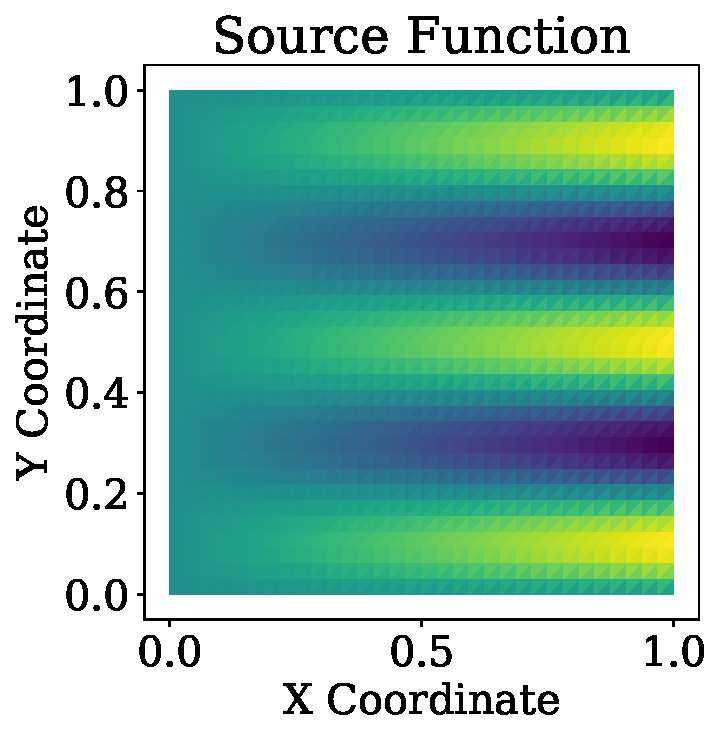
\includegraphics[width=0.32\textwidth]{./Images/Periodic/PeriodicSource1}
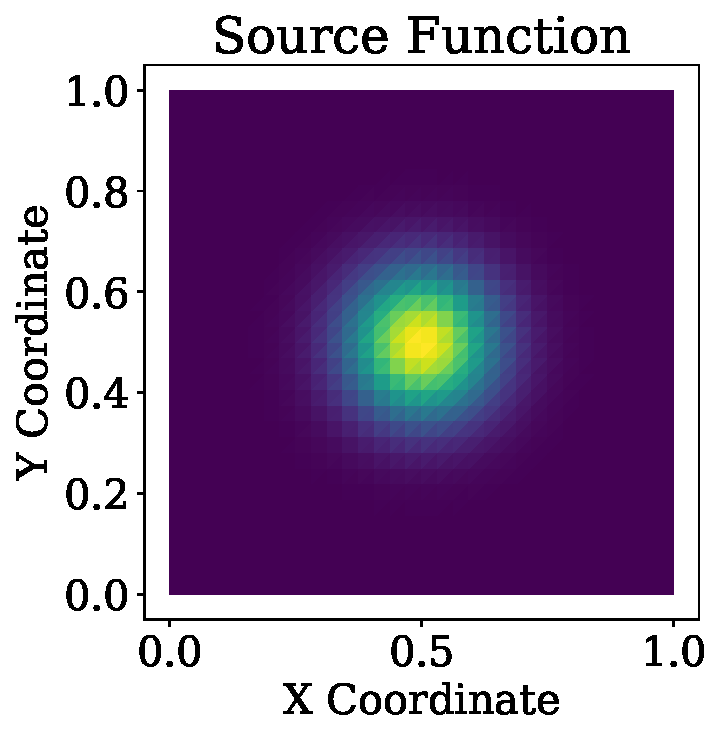
\includegraphics[width=0.32\textwidth]{./Images/Periodic/PeriodicSource2}
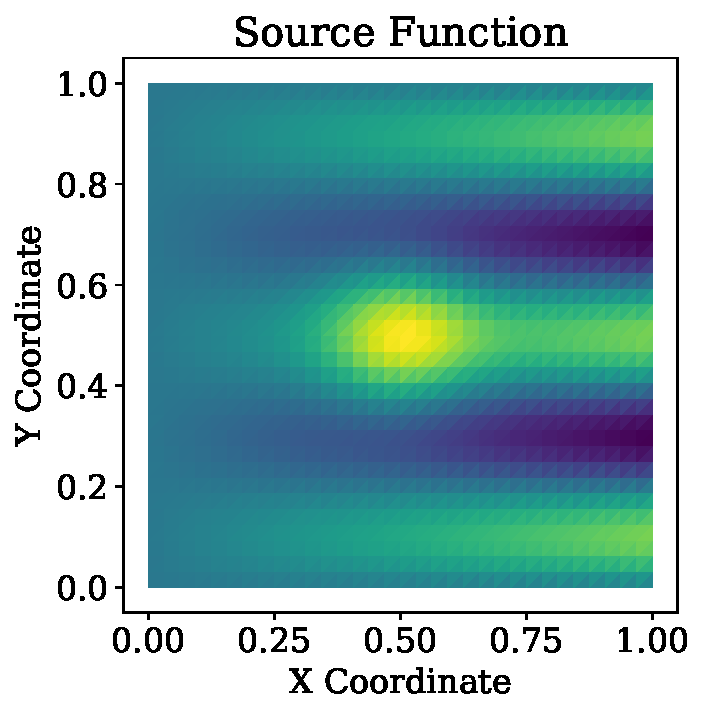
\includegraphics[width=0.32\textwidth]{./Images/Periodic/PeriodicSource}
\caption{Visualization of the source function A) first term in Eq. \ref{EqPeriodicSource}, the B) second term in Eq. \ref{EqPeriodicSource}, and C) the full source term, $f(x,y)$}
\label{FigSource}
\end{figure}

One key change made in order to prevent a warning message from appearing is adding the last two lines to the following class  to define the {\fontfamily{qcr}value\_shape \selectfont } \\ 
{\fontfamily{qcr}\selectfont
class Source(UserExpression): \\
\indent def eval(self, values, x): \\
 \indent\indent       dx = x[0] - 0.5 \\
\indent\indent        dy = x[1] - 0.5 \\
\indent\indent        values[0] = x[0]*sin(5.0*DOLFIN\_PI*x[1]) + ... \\
\indent    def value\_shape(self): \\
 \indent\indent        return () \\ \\
}
Lastly, some post-processing is included for visualization of the periodic boundary condition enforcement. This is left to give future users some idea of how to extract any field of interest. 


%=====================================================================
%=====================================================================
\subsection{Mixed Formulation for Poisson's Equation}
\vspace{-1ex}
In this version, I kept the original mesh, where N is a parameter for the number of elements in the x and y direction \\
{\fontfamily{qcr}\selectfont
mesh = UnitSquareMesh(N, N)  \\ \\
}
The notable part of the mixed formulation is given below \\
{\fontfamily{qcr}\selectfont
BDM = FiniteElement("BDM", mesh.ufl\_cell(), 1) \\
DG  = FiniteElement("DG", mesh.ufl\_cell(), 0) \\
W = FunctionSpace(mesh, BDM * DG) \\
}
where we find $(\bm{\tau}, \, u) \in (\Sigma_g \times V)$ which is the Brezzi-Douglas-Marini (BDM) and Discontinuous Galerkin (DG) space respectively. Stability of mixed elements is a complex topic, but the order of the BDM space must be higher than the DG space.  \\
{\fontfamily{qcr}\selectfont
(q, u) = TrialFunctions(W)
(tau, v) = TestFunctions(W) \\ \\
}
The boundary class wasn't working in the last stable FEniCS release; therefore, a fix is to specify different boundaries and expressions. The boundary must also be flipped from the previous definition since the Neumann BC now becomes the Dirichlet BC. \\
{\fontfamily{qcr}\selectfont
class BotBoundary(SubDomain): \\
 \indent def inside(self, x, on\_boundary): \\
 \indent\indent       return x[1] < DOLFIN\_EPS \\ \\
class TopBoundary(SubDomain): \\
 \indent   def inside(self, x, on\_boundary): \\
  \indent \indent      return x[1] > 1.0 - DOLFIN\_EPS \\ \\
}
It really isn't necessary to make these classes, but this is my own preference. We know that the normal to the bottom boundary is $\mathbf{n} = [ 0, -1]$ and the normal to the top boundary is $\mathbf{n} = [ 0, 1]$. The flux is meant to be enforced as a Dirichlet BC as $\mathbf{q} \cdot \mathbf{n} = g $. Therefore, we can write the following expressions and enforce them on the proper boundaries. An example is included below \\
{\fontfamily{qcr}\selectfont
g0 = Expression(("0", "sin(5*x[0])"), degree=2) \\
g1 = Expression(("0", "-sin(5*x[0])"), degree=2) \\
BotBC = DirichletBC(W.sub(0), g0, BotBoundary) \\
TopBC = DirichletBC(W.sub(0), g1, TopBoundary) \\
bc = [BotBC, TopBC] \\ \\
}
Note that we are using the same expressions in Eq. \ref{EqSourceBoundTerm} for this example. It is possible to further subclass the function space {\fontfamily{qcr}\selectfont W.sub(0).sub(0)} would indicate the x-dimension of the BDM subspace and {\fontfamily{qcr}\selectfont W.sub(0).sub(1)} would be the y dimension of the BDM subspace. An alternate way to define the above snippet of code would be the following.\\
{\fontfamily{qcr}\selectfont
g0 = Expression(("sin(5*x[0])"), degree=2) \\
g1 = Expression(("-sin(5*x[0])"), degree=2) \\
BotBC = DirichletBC(W.sub(0).sub(1), g0, BotBoundary) \\
TopBC = DirichletBC(W.sub(0).sub(1), g1, TopBoundary) 
}

\section{Results}
\vspace{-2ex}

\subsection{Periodic boundary condition results}
\vspace{-1ex}
To examine whether the periodic  was working properly, some post-processing is carried out where the solution profile on the right  and left boundary is plotted. As expected, Fig. \ref{FigPeriodicSolProfile}B demonstrates how the solutions match completely. Note that enforcement of periodicity, will not enforce a symmetric solution, as seen from the temperature solution as well as the plots of the profiles a small distance inwards from the right and left boundaries. 
\begin{figure*}[!htb]
\centering
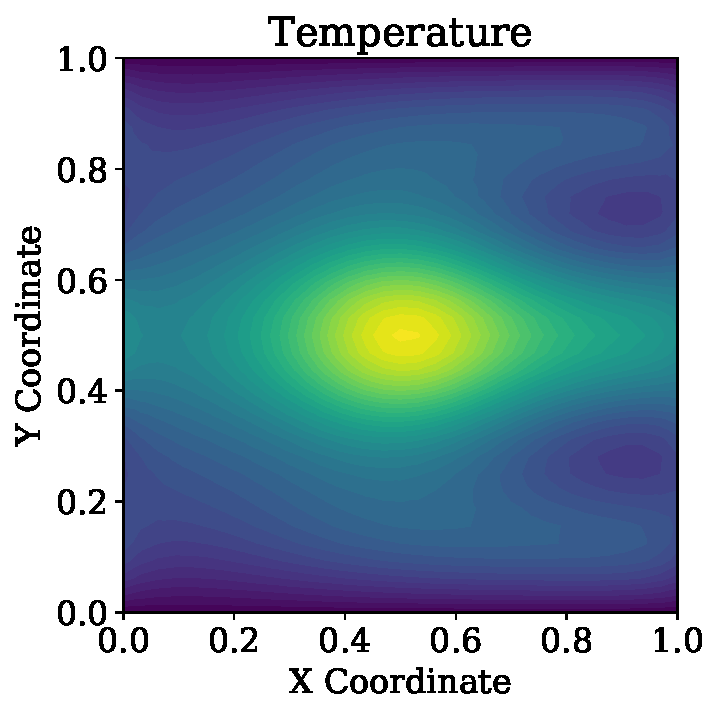
\includegraphics[width=0.32\textwidth]{./Images/Periodic/PeriodicTemp}
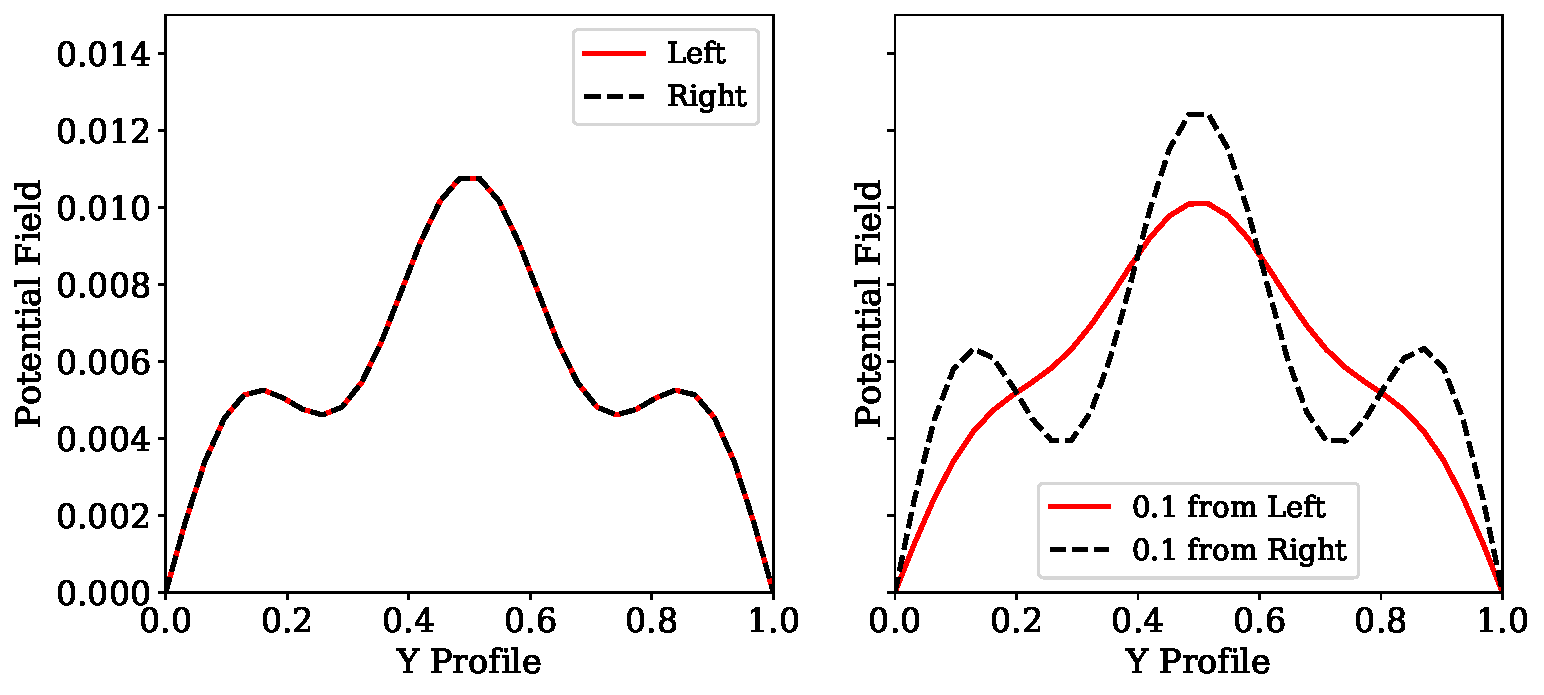
\includegraphics[width=0.65\textwidth]{./Images/Periodic/PeriodicSolProfile}
\caption{ Temperature or potential field results. A) Potential field within the domain. B) Solution profiles on the right and left boundaries. C) Solution profiles a distance 0.1 inwards from the right and left boundaries.  }
\label{FigPeriodicSolProfile}
\end{figure*}

\clearpage

\subsection{Comparison of single and mixed formulation}
\vspace{-1ex}

Fig. \ref{FigPoissonTemp} shows that the scalar temperature field for the results related to the first and third demonstration look quite similar, with some minor differences. 
\begin{figure*}[!htb]
\centering
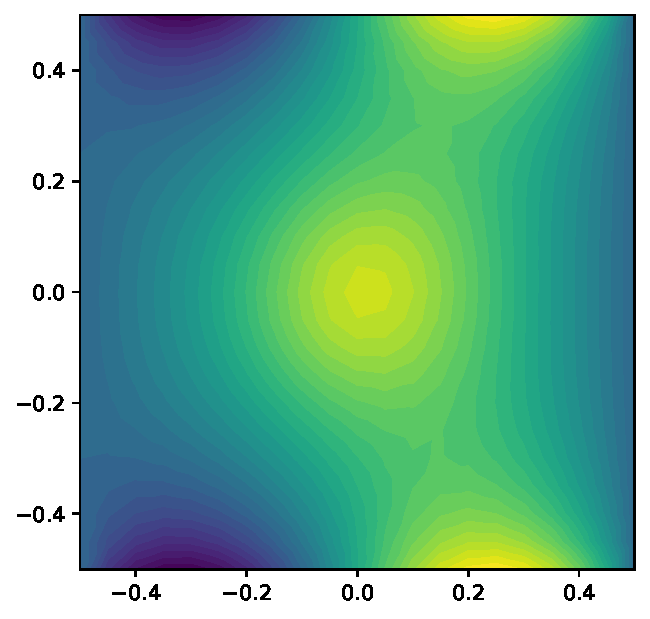
\includegraphics[width=0.35\textwidth]{./Images/Poisson//Temperature.pdf}
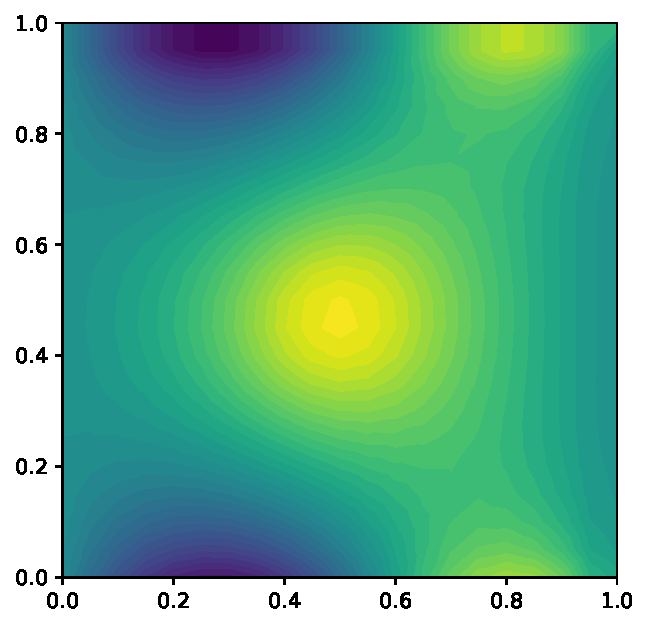
\includegraphics[width=0.35\textwidth]{./Images/PoissonMixed/Temperature.pdf}
\caption{General Solution or temperature results from Poisson formulation and mixed Poisson Formulation respectively.}
\label{FigPoissonTemp}
\end{figure*}

Fig. \ref{FigMixedPoisson} displays the temperature and heat flux results from the mixed Poisson formulation
\begin{figure*}[!htb]
\centering
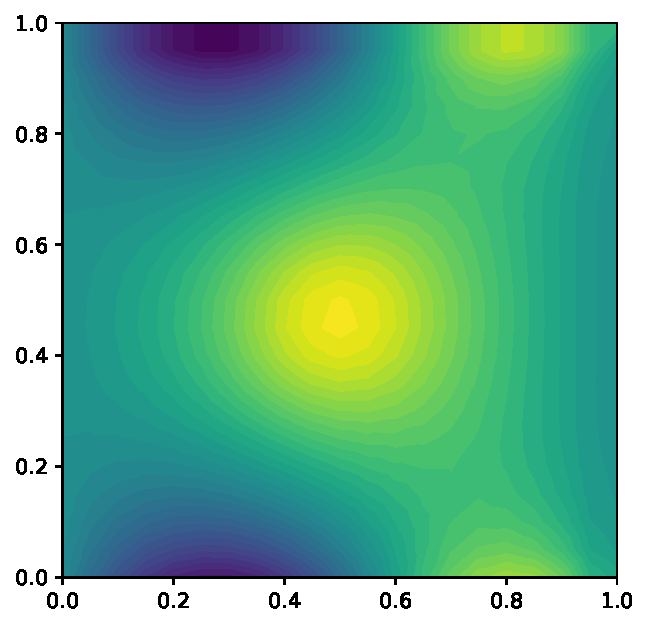
\includegraphics[width=0.35\textwidth]{./Images/PoissonMixed/Temperature.pdf}
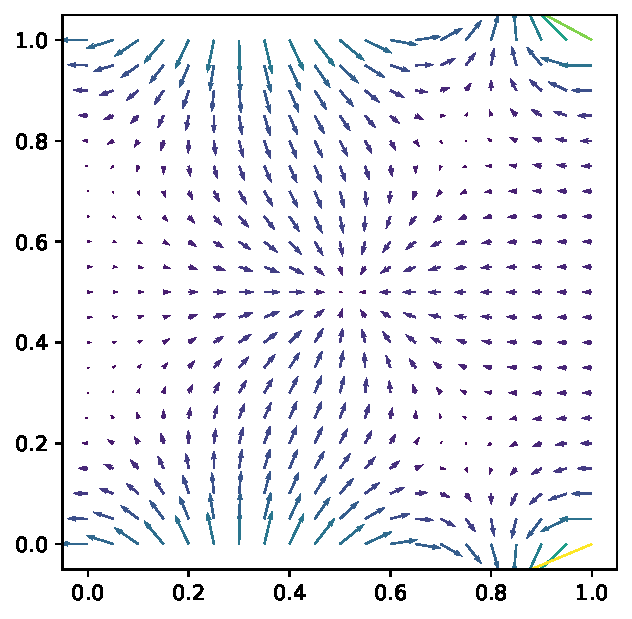
\includegraphics[width=0.35\textwidth]{./Images/PoissonMixed/HeatFlux.pdf}
\caption{Mixed Poisson formulation results for a) temperature and b) heat flux.  }
\label{FigMixedPoisson}
\end{figure*}


\end{document}
